Modify Program 13 so that instead of polyval and polyfit, it uses the more stable formula of barycentric
interpolation

$$p(x)=\sum_{j=0}^N\frac{a_j^{-1}u_j}{x-x_j}/\sum_{j=0}^N\frac{a_j^{-1}}{x-x_j}$$

where $\{a_j\}$ are defined by (6.7). Experiment with various interpolation problems (such as that of
Exercise 5.1) and find evidence of the enhanced stability of this method.\\\\

\begin{solution}\renewcommand{\qedsymbol}{}\ \\
    Using the barycentric interpolation, we have the following code. We test it with three different
    conditions for our ODE and get these three graphs. We can see that this interpolation method works
    well and is quite robust.

    \begin{figure}[htp]
        \centering
        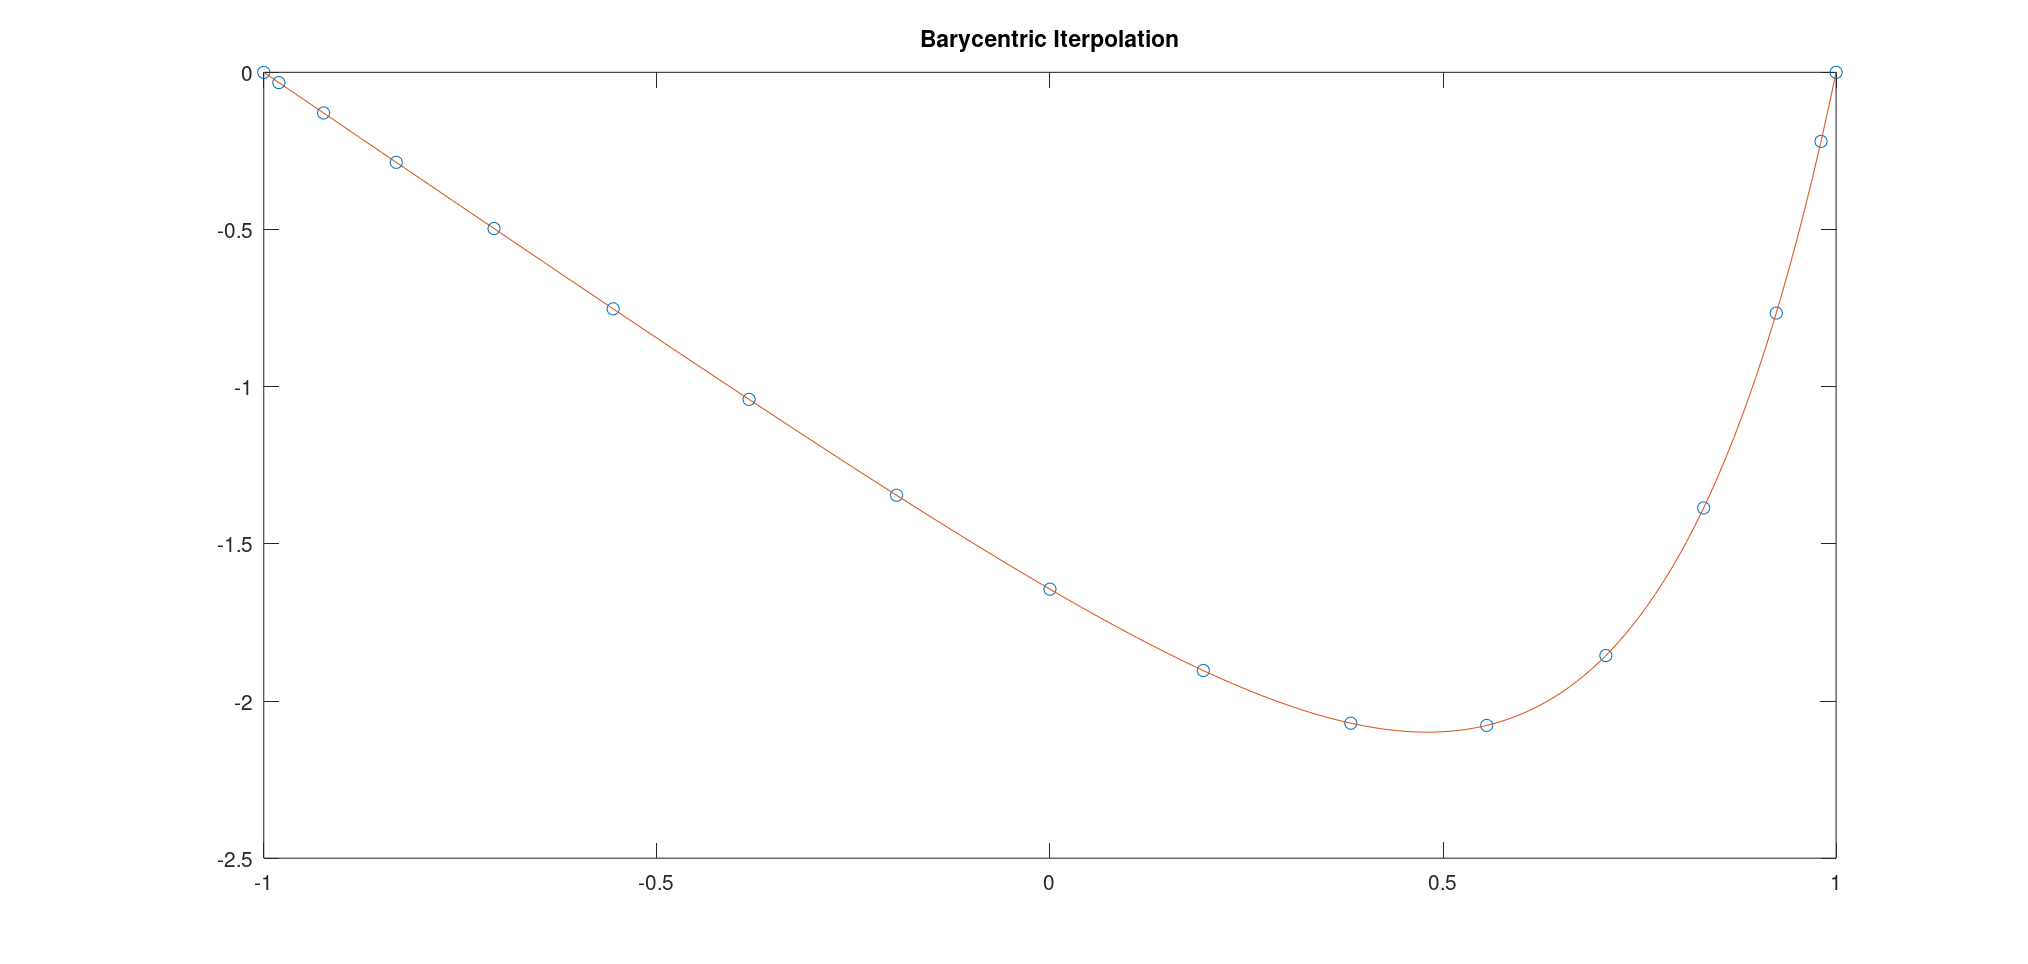
\includegraphics[scale=0.2]{7_1exp.PNG}
        \caption{$e^{4x}$}
    \end{figure}
    \begin{figure}[htp]
        \centering
        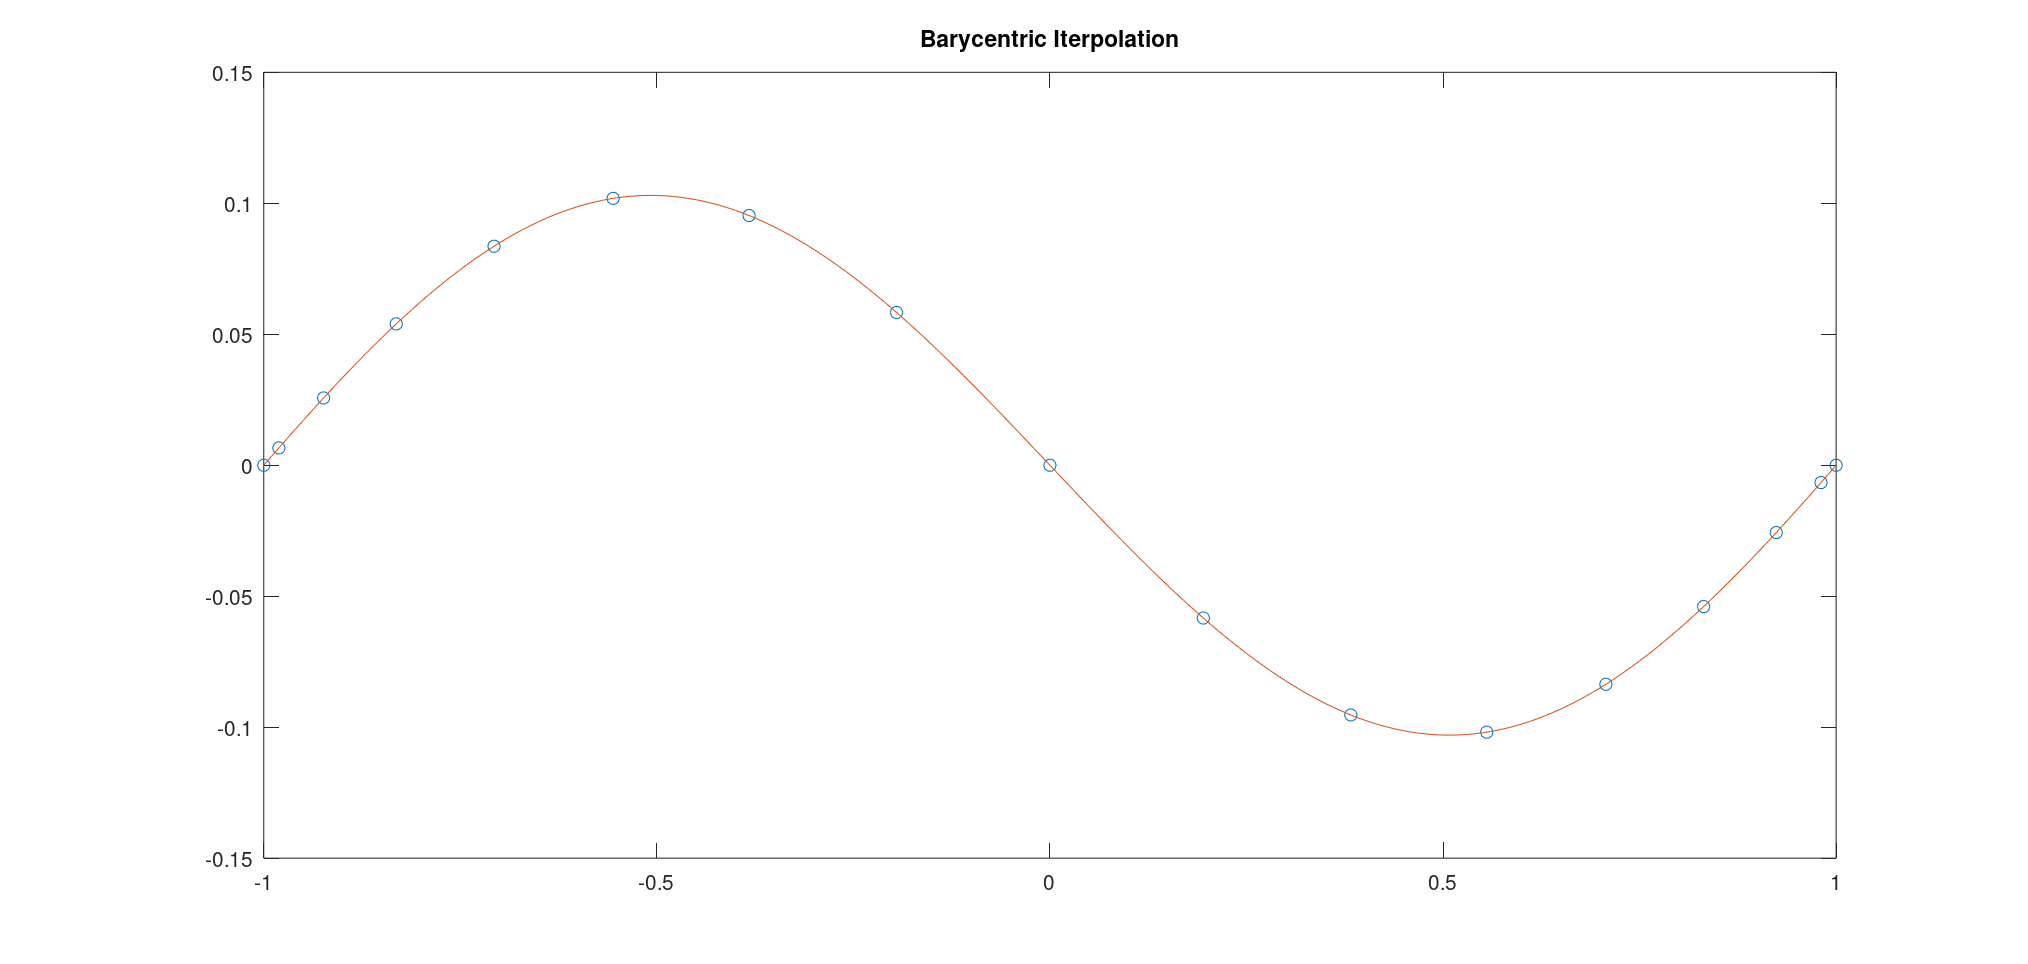
\includegraphics[scale=0.2]{7_1sin.PNG}
        \caption{$\sin(x)$}
    \end{figure}
    \begin{figure}[htp]
        \centering
        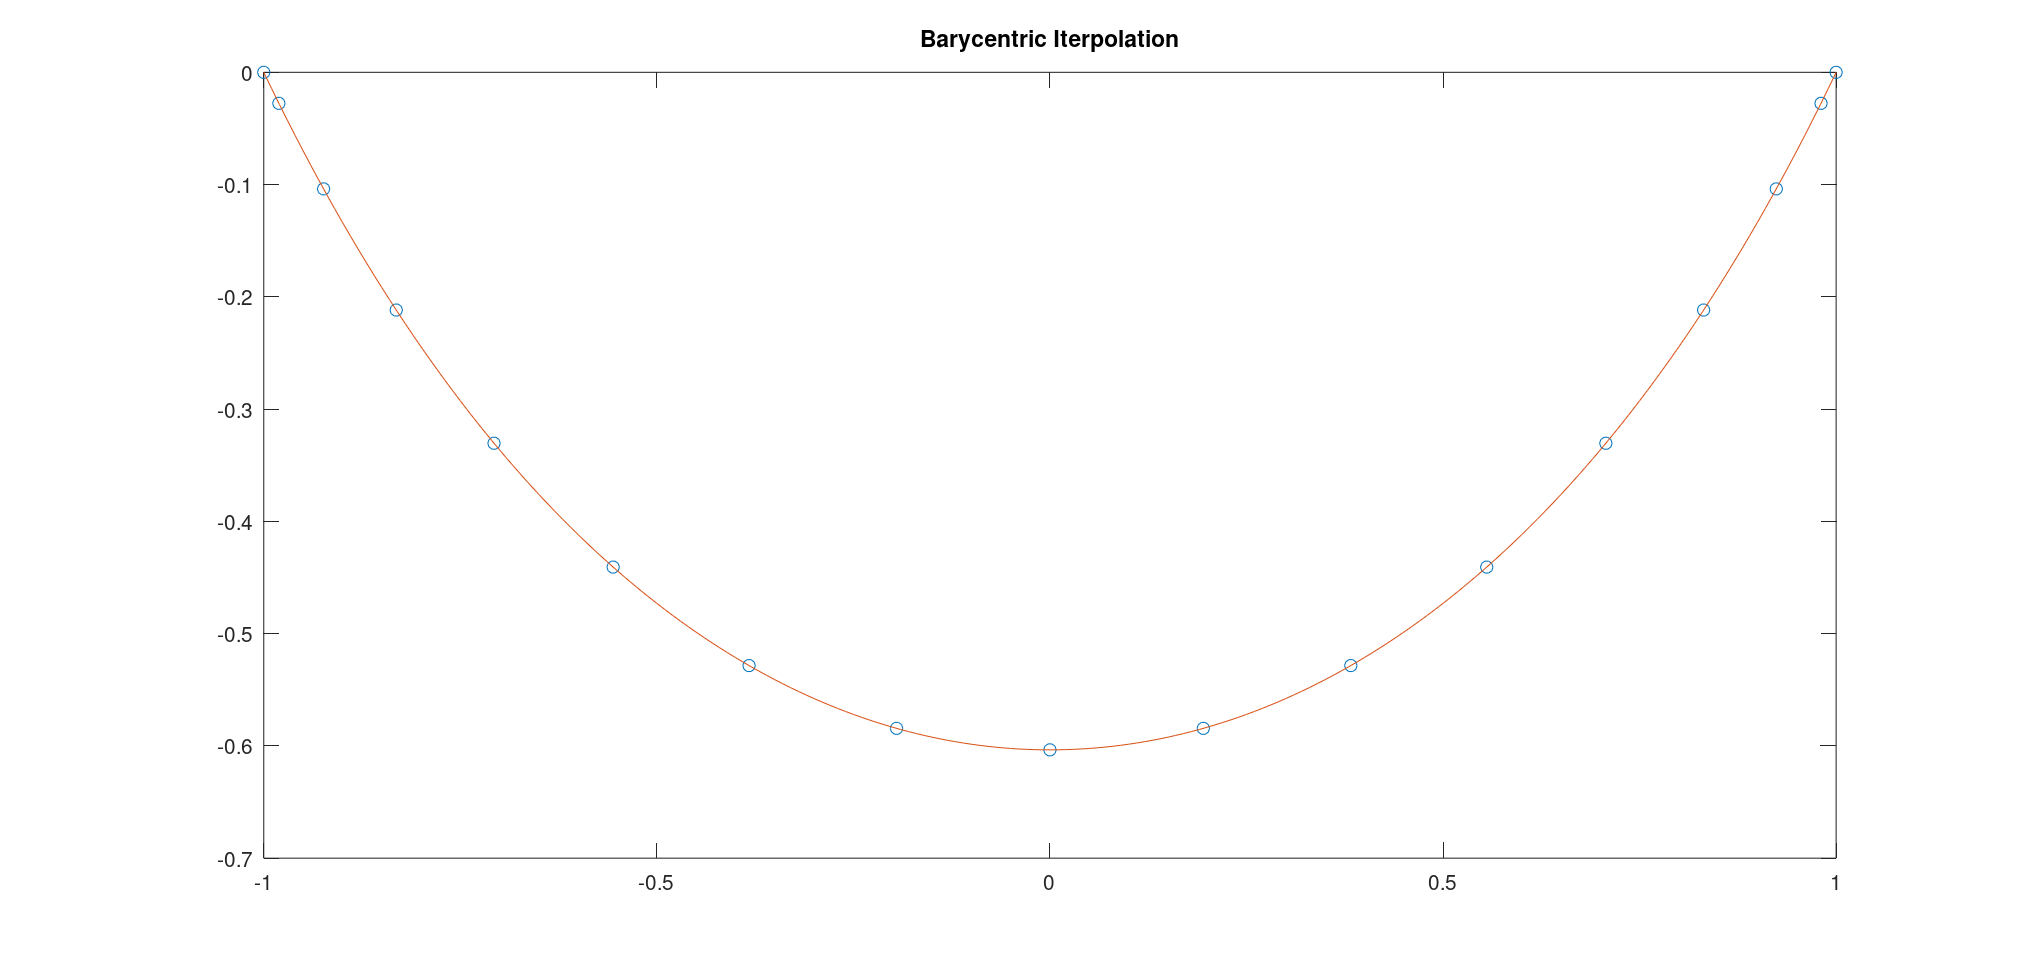
\includegraphics[scale=0.2]{7_1exp2.PNG}
        \caption{$e^{x^2}$}
    \end{figure}

\end{solution}

\newpage
\lstinputlisting{problem7_1.m}
\newpage